\documentclass{article}
\usepackage{ctex}
\usepackage{makecell}
\usepackage{graphicx}
\usepackage{geometry}
\usepackage{multirow}
\usepackage{multicol}
\usepackage{fancyhdr}
\usepackage{longtable}
\usepackage{color}
\usepackage{float}
\usepackage{listings}
\usepackage{xcolor}
\usepackage{hyperref}
\usepackage{footnote}
\usepackage{paralist}

\let\itemize\compactitem
\let\enditemize\endcompactitem
\let\enumerate\compactenum
\let\endenumerate\endcompactenum
\let\description\compactdesc
\let\enddescription\endcompactdesc

\geometry{a4paper,left=25mm,right=20mm,top=25mm,bottom=25mm}

\title{第四周周五实验}
\author{09021227~金桥}
\date{\today}

\lstset{
    numbers=left,
    keywordstyle= \color{ blue!70},
    commentstyle= \color{red!50!green!50!blue!50},
    rulesepcolor= \color{ red!20!green!20!blue!20} ,
    % escapeinside=``,
    numberstyle=\tt,
    numbersep=0em,
    xleftmargin=2em,
    breaklines,
    aboveskip=1em,
    framexleftmargin=2em,
    frame=shadowbox,
    basicstyle=\tt,
    language=C++
}

\begin{document}

\maketitle

\section{实验目标}

在第一次实验作业的基础上,搭建一个可视化界面,实现对幻灯片中磁共振膝盖图像进行傅立叶变换、直方图表示、直方图均衡化、CLAHE算法结果的展示,并体现自己的思考过程。

\section{实验内容}

\subsection{傅里叶变换}

傅里叶变换已经在第一次实验中实现,参见实验报告一。

\subsection{显示直方图}

\subsubsection{使用OpenCV计算直方图}

通过调用 OpenCV 提供的 \texttt{calcHist} 函数可以方便快速的实现直方图计算。
具体调用参见代码。

\subsubsection{自行计算直方图}

计算过程如下,具体实现参见代码。

\begin{itemize}
    \item 首先使用\texttt{cvtColor}函数将原图像转为灰度图
    \item 之后通过\texttt{cvt2dVector}函数将\texttt{Mat}格式的图像转换为\texttt{int}格式的二维\texttt{vector}
    \item 之后遍历所有像素,统计不同灰度像素点数量
    \item 最后将统计结果绘图
\end{itemize}

\subsection{直方图均衡}

\subsubsection{使用OpenCV进行直方图均衡}

通过调用 OpenCV 的 \texttt{equalizeHist} 函数可以方便快速的实现直方图均衡。
具体调用参见代码。

\subsubsection{自行直方图均衡}

计算过程如下,具体实现参见代码。

\begin{itemize}
    \item 首先使用之前的计算直方图的步骤计算直方图
    \item 之后根据直方图数值计算累计分布函数,并进行归一化
    \item 根据计算出来的累计分布函数将原来的图像灰度映射到新的灰度上
\end{itemize}

\subsection{CLAHE算法}

\subsubsection{使用OpenCV实现CLAHE}

通过调用 OpenCV 提供的 \texttt{CLAHE} 类可以方便快速的实现CLAHE算法。
具体调用参见代码。

\subsubsection{自行实现CLAHE}

计算过程如下,具体实现参见代码。

\begin{itemize}
    \item 首先将图像分块(OpenCV默认$8\times 8$分块, 与其保持一致),图像边缘不够的进行补齐
    \item 对每个分块进行处理:
    \begin{itemize}
        \item 计算出分块的直方图数值
        \item 根据预设的阈值对直方图进行裁切,将高处的部分均匀补齐至所有灰度上
        \item 返回处理后的直方图
    \end{itemize}
    \item 为防止棋盘效应对图像造成割裂,采用双线性插值
    \begin{itemize}
        \item 对每个块的像素,取离它最近的四个分块,并取出四个分块处理后对应的灰度值
        \item 假设从上到下,从左到右,四个灰度值分别是 $r_1, r_2, r_3, r_4$
        \item 假设在离这个像素最近的四个分块的中心点形成的矩形中:
        \begin{itemize}
            \item 这个像素距离上下边界的距离是 $y_1, y_2$,左右边界距离 $x_1, x_2$,分块横纵大小 $w, h$
        \end{itemize}
        \item 代入下式计算最终像素灰度$r$:$$r = (r_1 \frac{x_1}{w} + r_2 \frac{x_2}{w})\frac{y_1}{h} + (r_3 \frac{x_1}{w} + r_4 \frac{x_2}{w})\frac{y_2}{h}$$
    \end{itemize}
\end{itemize}

\section{实验结果}

\subsection{显示直方图}

直方图显示采用的是自行实现的算法。

\begin{figure}[H]
    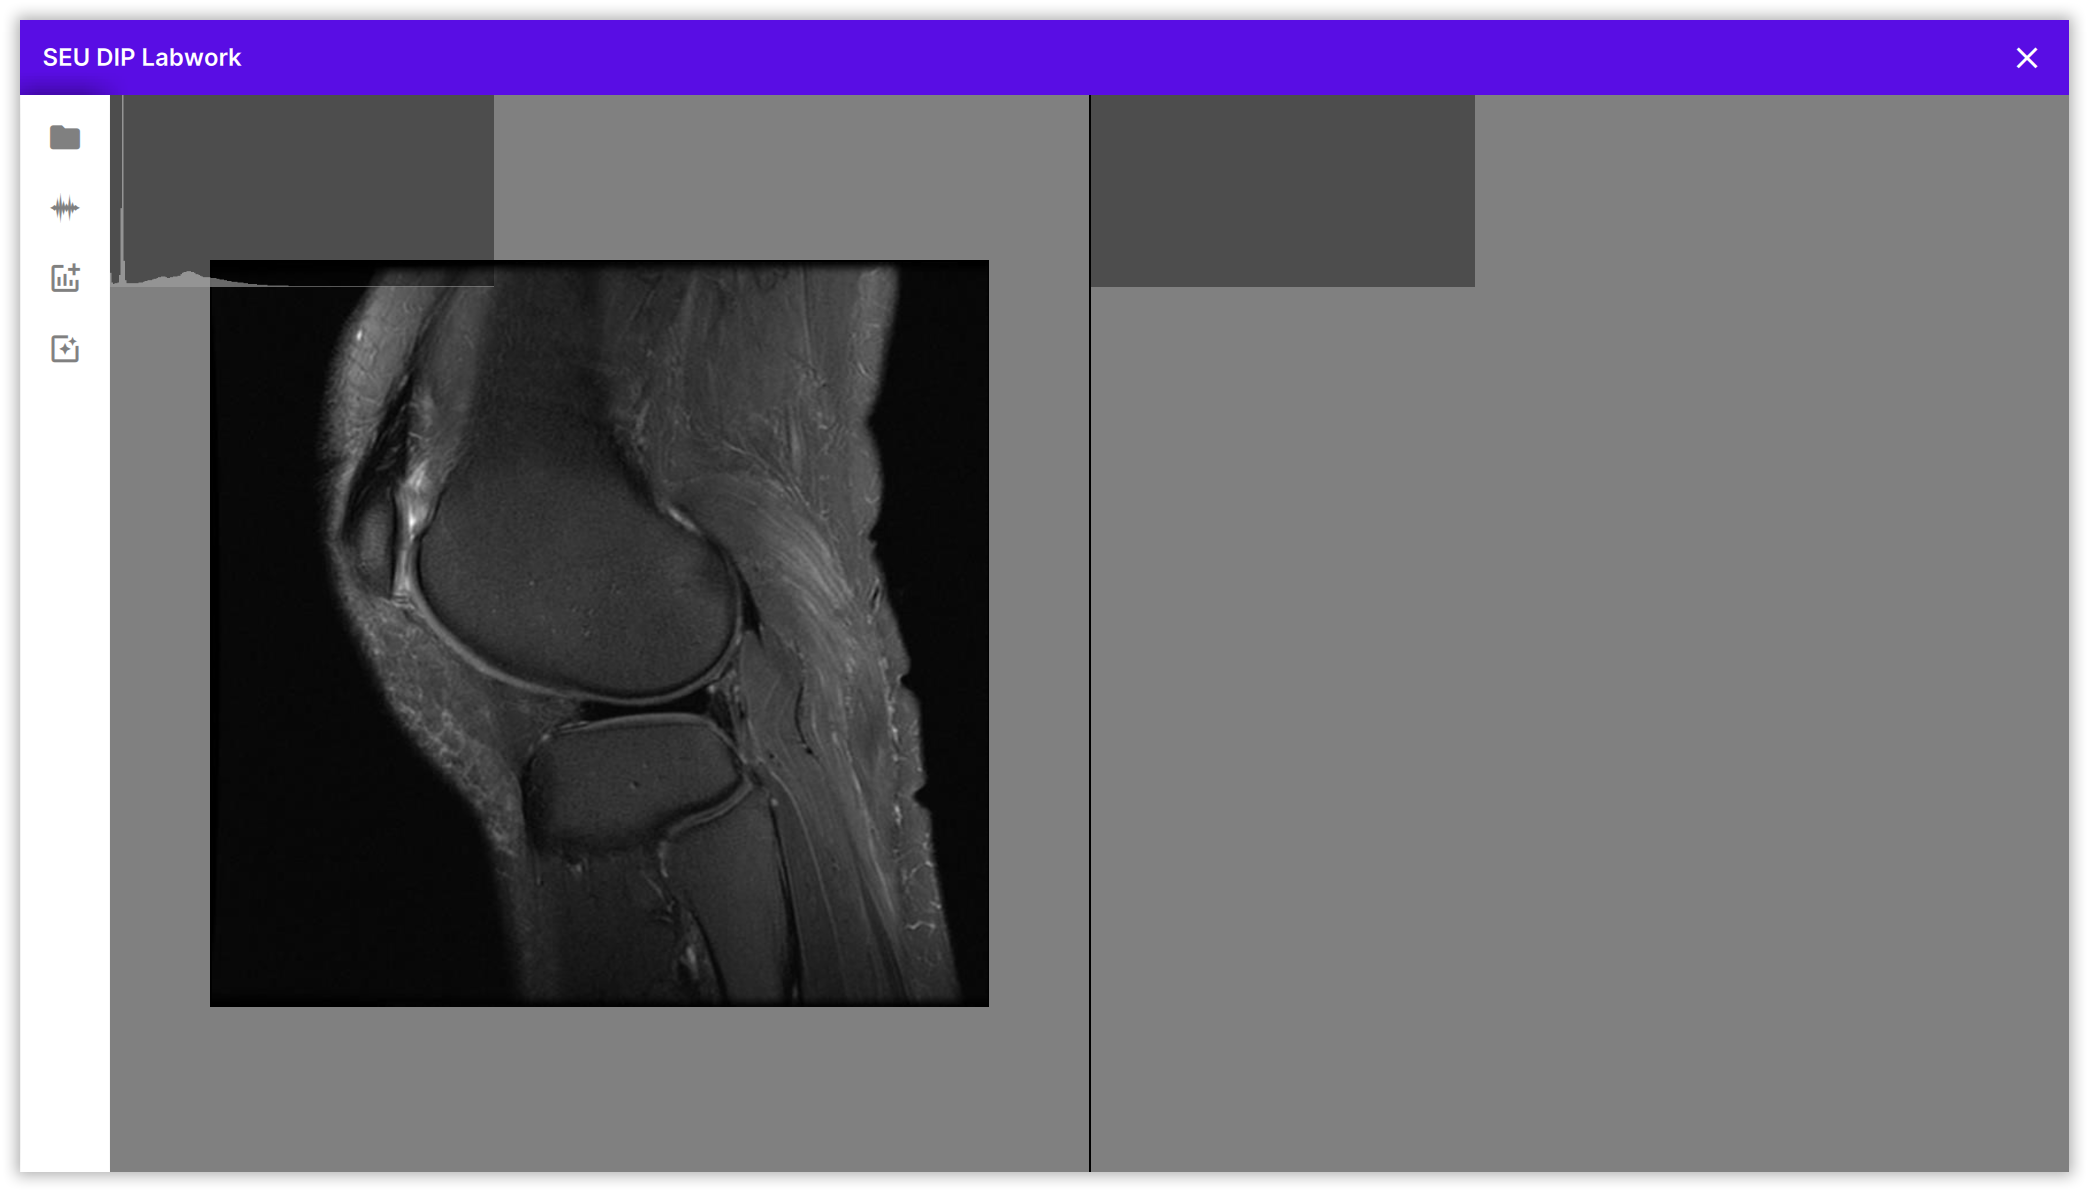
\includegraphics[width=\textwidth]{img/histo_disp.png}
\end{figure}

\subsection{直方图均衡}

下图是自行实现的直方图均衡算法。

\begin{figure}[H]
    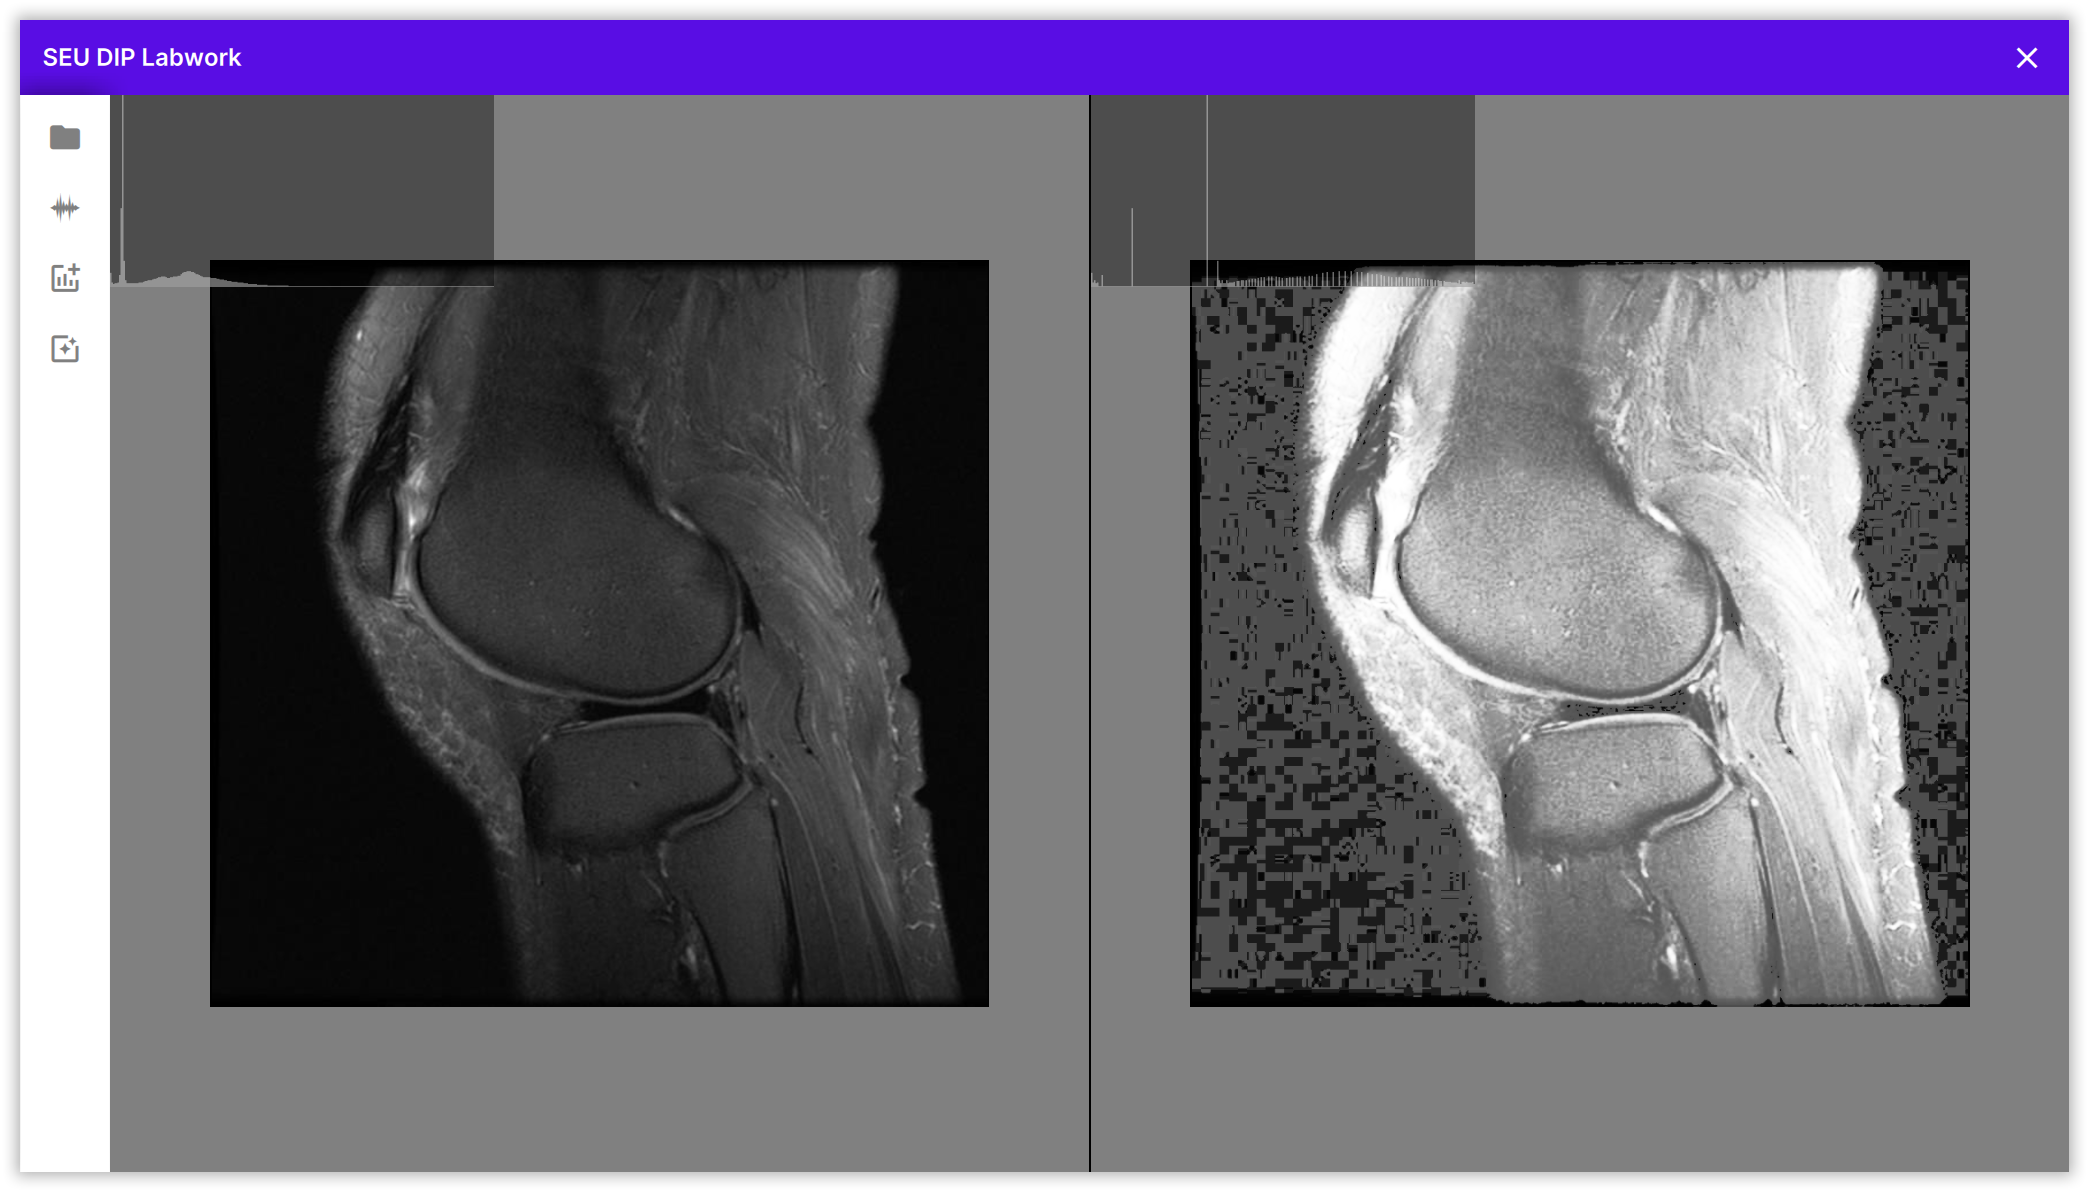
\includegraphics[width=\textwidth]{img/histo_equ.png}
\end{figure}

\subsection{CLAHE算法}

下图是自行实现的CLAHE算法。

\begin{figure}[H]
    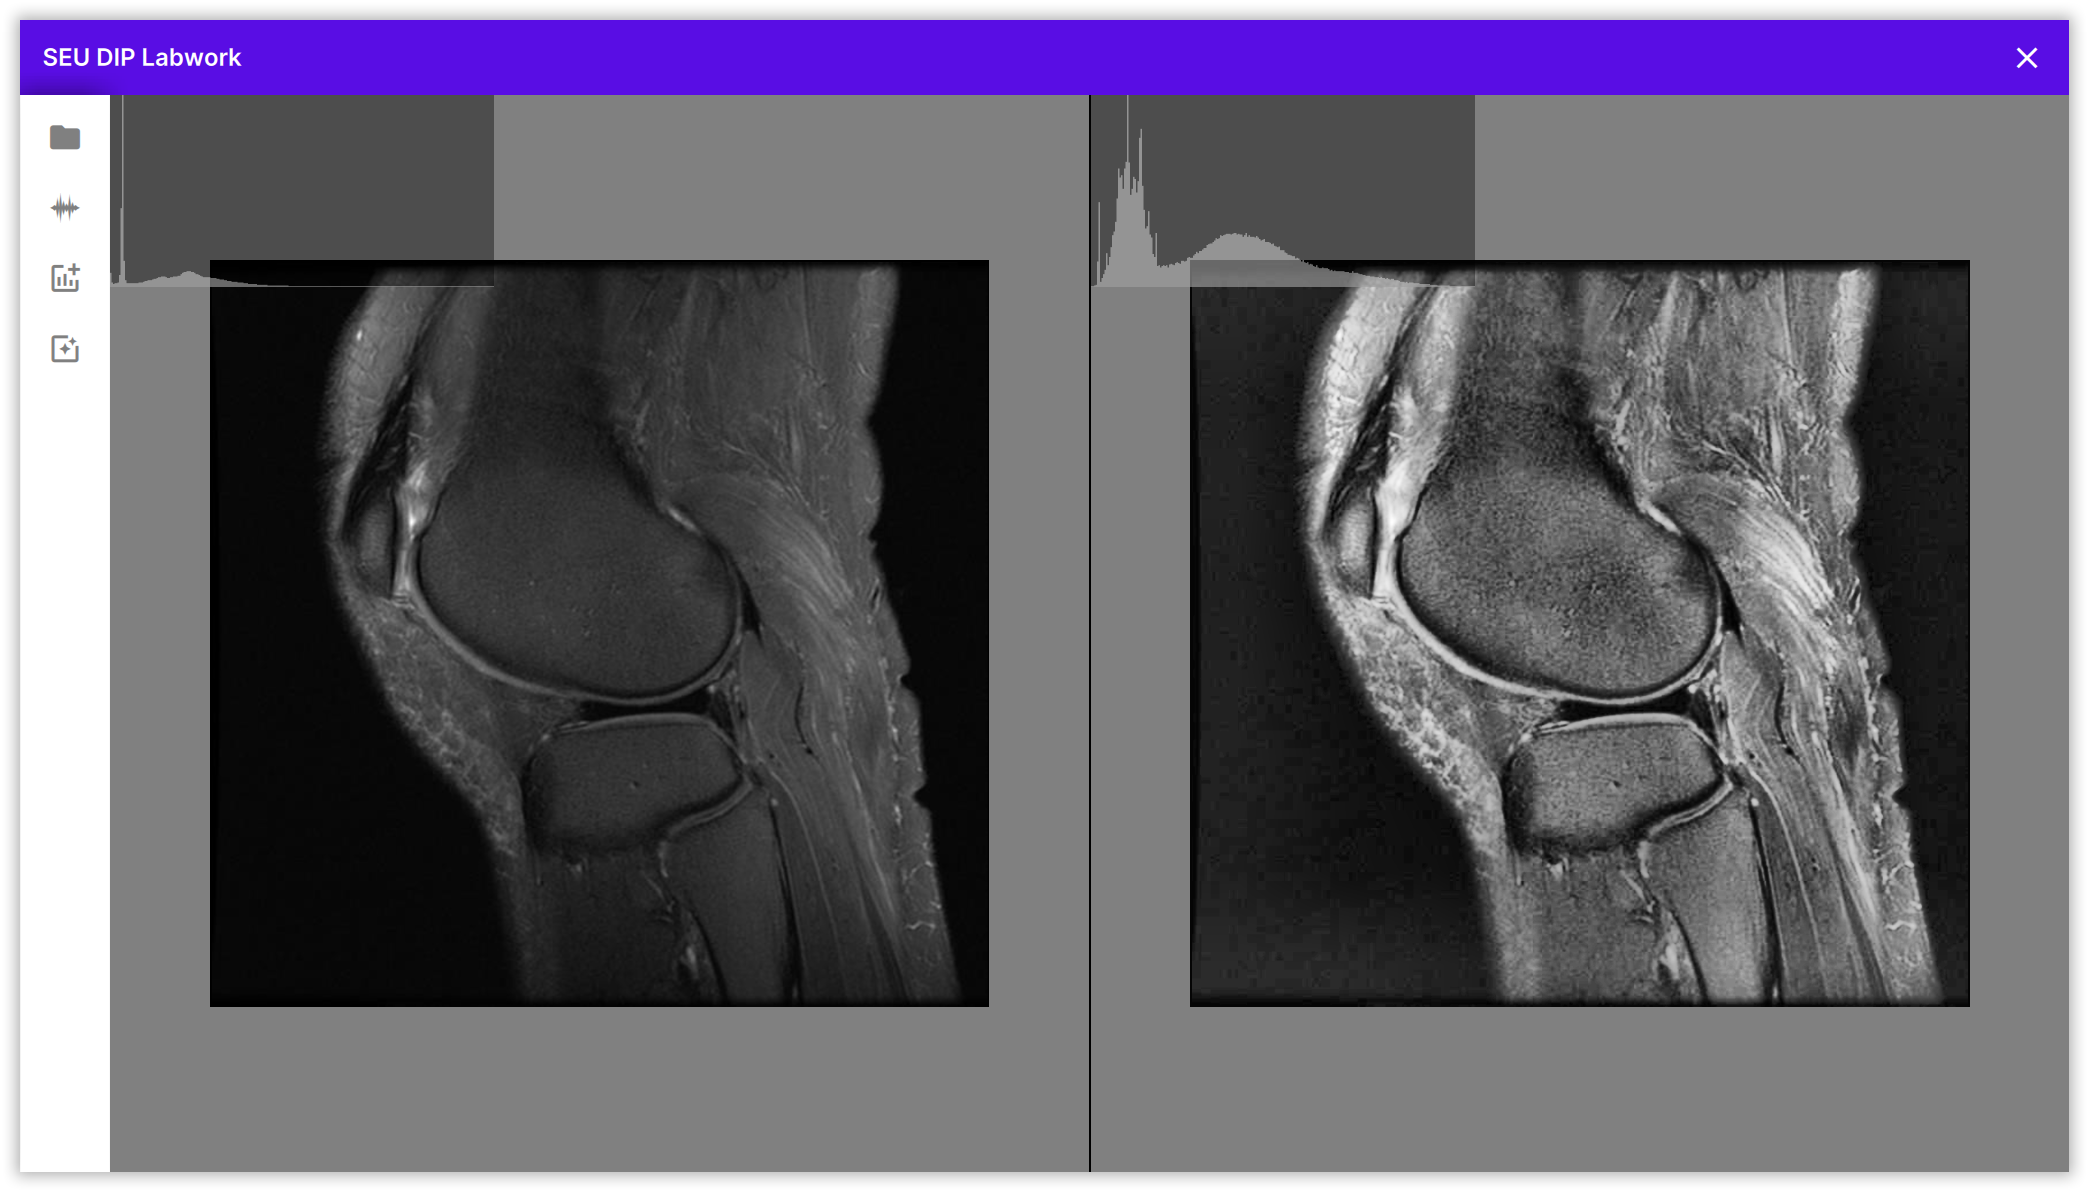
\includegraphics[width=\textwidth]{img/clahe.png}
\end{figure}

\section{思考}

\subsection{为什么OpenCV的傅里叶变换速度比较快?}

作为对比,我自行实现的傅里叶变换的时间复杂度大约是 $O(m^2n^2)$ 而 OpenCV 的傅里叶变换速度极快,几乎是瞬间实现的。查阅资料后,发现主要原因有以下两个:

1. OpenCV 大量运用了并行计算,对于傅里叶变换这种大量\texttt{for}循环的算法具有显著的优势

2. OpenCV 的傅里叶变换采用的是快速傅里叶变换,而我采用的是离散傅里叶变换,虽然结果基本一致但在时间复杂度上差了一个量级

\subsection{直方图相关算法结果细微差异原因}

对于直方图相关算法,我的实现与OpenCV的实现产生的结果有非常细微的差别,经过分析,我认为主要原因是对于浮点数转为整数,我采用的是向下取整,而OpenCV采用的是四舍五入取整,因此会有非常细微的差别。


\subsection{CLAHE对比HE的优势}

CLAHE相对于HE的优势主要是它不会产生过度的增强,在改善整体图像对比度的同时不会过度增强某些区域的对比度,从而避免图像细节丢失。

我个人认为这主要得益于CLAHE有\texttt{clipLimit}的设置,可以防止过度增强对比度。除此以外,CLAHE的分块计算也在一定程度上保留了局部图像的对比度。

\end{document}
